\message{ !name(index.tex)}\documentclass[11pt]{article}                                                   
\usepackage[colorlinks]{hyperref}                                               
\usepackage{breakurl}                                                           
\usepackage{amsmath}                                                            
\usepackage[margin=.9in]{geometry}                                              
\newcommand{\nx}{\texttt{quigley}}                                              
\newcommand{\sechost}{\texttt{secureIpums}}                                     
\newcommand{\repo}{\texttt{/home/ipums-repo}}                                   
\newcommand{\ipums}{\texttt{$\sim$/IPUMS}}                                      
%\newcommand{\uP}{$\square$}                                                    
\newcommand{\ar}{$\rightarrow$}                                                 
\newcommand{\user}[1]{\texttt{#1}}                                              
\usepackage{mdframed}                                                           
%\usepackage{color}                                                             
%\usepackage{framed}                                                            
\usepackage{xcolor}       
\usepackage{graphicx}
\begin{document}

\message{ !name(index.tex) !offset(-3) }


\title{The Rstudio175 cloud server\\
for Demog/Econ C175}

\maketitle
\tableofcontents

\section{Introduction}

The Rstudio175 cloud server is the computing infrastructure for all of the homework assignments in Demog/Econ 175. If you are not enrolled in this course, please hang up and dial 9-1-1.
\begin{mdframed}[backgroundcolor=blue!20]        
\textbf{There are two ways to use Rstudio}. We recommend using the \textbf{cloud server} described below, however, it is also possible to install the \textbf{desktop} version of  Rstudio on your own machine and download the homework files from \url{http://courses.demog.berkeley.edu/goldstein175}. If you choose the Desktop plan, you are pretty much on your own.
\end{mdframed}
\section{Getting started}

Shortly after registering for C175, you should recieve email with instructions on how to initialize your account by setting your password.  All you should need to do is click on the link included in the email, and provide a new password.  If you never reieved this email verify that you are registered, then send email to trouble@demog.berkeley.edu.  Note that you must initialize your account within two weeks of the start of the semester to avoid administrative hurdles.

Once you have established a password for your Rstudio175 Cloud account, go to 
\url{http:courses.demog.berkeley.edu/goldsein175} and click on the large obvious button labeled ``Launch Rstudio175 Cloud'' to launch the Rstudio175 cloud.

You should soon be confronted with a web page sporting the Rstudio login dialog:

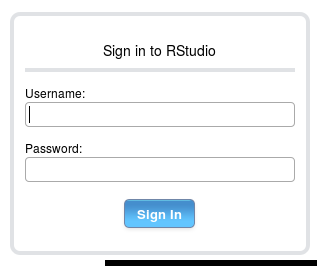
\includegraphics[scale=.35]{RstudioSignin}

Your username, (as indicated in the above mentioned email) is your calnet ID but your
password is whatever you set it to be.  


\end{document}

\message{ !name(index.tex) !offset(-52) }
